\documentclass[11pt]{article}

\usepackage[margin=1in]{geometry}
\usepackage{amsmath,amssymb,amsthm}
\usepackage{booktabs}
\usepackage{graphicx}
\usepackage[hidelinks]{hyperref}

\setlength{\parskip}{0.45em}
\setlength{\parindent}{0pt}
\setlength{\emergencystretch}{1.5em}
\widowpenalty=10000
\clubpenalty=10000

\newtheorem{theorem}{Theorem}
\newtheorem{proposition}[theorem]{Proposition}
\newtheorem{remark}[theorem]{Remark}

\newcommand{\clip}{\operatorname{clip}}
\newcommand{\ind}{\mathbf{1}}

\title{\textbf{Online vs.\ Rolling Statistical Jump Models:\\
Bounded-Score Coalescence and Delay-Budget Penalty Calibration}}

\author{Tan Le\\[3pt]
\small Knox College $\cdot$ \texttt{lethongtan4@gmail.com}}
\date{November 2026}

\begin{document}
\maketitle

\begin{abstract}
Statistical Jump Models (SJMs) segment noisy time series into persistent regimes by charging a fixed penalty $\lambda \ge 0$ for each state transition. When deployed in real time, however, practitioners face two unresolved design choices: (i) whether to propagate dynamic-programming arrival costs continuously from the start of the stream (\emph{carried-score} online decoding, as implemented in \texttt{jumpmodels.predict\_online}) or re-solve a sliding window of $W$ observations at each step (\emph{rolling-$W$} terminal decoding), and (ii) how to choose $\lambda$ when neither ground-truth regime labels nor downstream trading payoffs are available. Using an elementary one-dimensional clipped-score representation of the two-state dynamic program, we prove three short results. First, carried-score and rolling-$W$ trajectories contract monotonically and \emph{coalesce identically} whenever the shared window hits either clipping barrier $\pm\lambda$, whereas short rolling windows can double emitted switching rates when $\lambda$ increases even as internal window jumps fall to zero. Second, for fitted centroids separated by per-step loss $\Delta = \frac{1}{2}\|\mu_1 - \mu_0\|_2^2 > 0$, we derive exact worst-case step-response delays $d_{0\to 1}(\lambda) = \lfloor \lambda/\Delta \rfloor + 1$ and $d_{1\to 0}(\lambda) = \max(1, \lceil \lambda/\Delta \rceil)$, yielding the sharp feasibility bound $\lambda < B\Delta$ for any operational delay budget $B \ge 1$. Third, we implement these results in a lightweight, dependency-minimal Python package (\texttt{jm-online}) compatible with \texttt{jumpmodels}. Across three out-of-sample public monitoring benchmarks---smart-building HVAC sensors (UCI Occupancy, 12,417 minutes), urban air-quality alerts (Beijing PM2.5, 17,520 hours), and financial volatility stress monitoring (CBOE VIX, 5,038 trading days)---delay-budget calibration reduces false regime switching by $66\%$--$75\%$ without labels, preserves a $1.0$-minute median arrival lag on held-out camera ground truth, and confirms exact $0.00\%$ carried-versus-rolling coalescence at moderate window lengths.
\end{abstract}

\section{Introduction}

Real-time monitoring systems---such as demand-controlled building ventilation, urban air-pollution advisories, and financial market risk dashboards---must classify noisy multivariate observations $x_t \in \mathbb{R}^p$ into discrete operating regimes without excessive flickering. Unpenalized clustering reacts immediately to single-step noise, causing actuator wear and alarm fatigue. Statistical Jump Models \cite{bemporad2018,nystrup2020} address this instability by combining pointwise clustering loss with a fixed penalty $\lambda \ge 0$ per state transition:
\begin{equation}
  J_\lambda(s_{1:T}) \;=\; \sum_{t=1}^{T} \ell_t(s_t) \;+\; \lambda \sum_{t=2}^{T} \ind\{s_t \ne s_{t-1}\},
  \qquad \ell_t(k) = \tfrac{1}{2}\|x_t - \mu_k\|_2^2.
  \label{eq:sjm}
\end{equation}
Offline decoding minimizes \eqref{eq:sjm} over the entire record $x_{1:T}$ via Viterbi dynamic programming, which uses future observations $x_{t+1:T}$ to smooth past labels. Real-time decisions at step $t$, by contrast, may use only $x_{1:t}$.

Inspection of recent literature and the reference Python package \texttt{jumpmodels} \cite{shu2024} reveals two practical gaps in real-time SJM deployment:
\begin{enumerate}
  \item \textbf{Carried-score streaming vs.\ rolling-$W$ reset windows.} In \texttt{jumpmodels}, the method \texttt{predict\_online} propagates forward dynamic-programming values indefinitely from $t = 1$ and emits the current argmin (\emph{carried-score} decoding). Empirical studies, however, frequently describe online inference as re-optimizing \eqref{eq:sjm} from scratch on a trailing window of length $W$ and emitting only its final label (\emph{rolling-$W$} decoding; e.g., \cite[Sec.~3.4.2]{shu2024}). When do these two causal decoders agree, and when do they diverge?
  \item \textbf{Label-free calibration of $\lambda$ without backtest overfitting.} Existing tuning strategies select $\lambda$ either by cross-validating downstream portfolio Sharpe ratios \cite{nystrup2020,shu2024}---which is inapplicable outside trading and prone to historical overfitting---or via offline information criteria \cite{cortese2026} that count internal jumps of a single offline fit rather than online switching versus detection latency. In \texttt{jumpmodels}, no penalty selector is provided.
\end{enumerate}

This paper resolves both questions with short, self-contained algebraic proofs and an open-source Python companion library (\texttt{jm-online}). Section~\ref{sec:theory} reduces two-state causal decoding to a one-dimensional clipped recursion, proves exact trajectory coalescence between carried-score and rolling-$W$ decoders once a window saturates either $\pm\lambda$ barrier, and exhibits an explicit eight-step cycle on which increasing $\lambda$ drives internal window jumps to zero while \emph{doubling} rolling-$7$ emitted switches. Section~\ref{sec:calibration} derives exact directional step-response delays for real-valued centroids and turns any user-specified delay budget $B$ into a closed-form penalty ceiling $\lambda < B\Delta$. Section~\ref{sec:experiments} validates both mechanisms out of sample on three public sensor and risk-monitoring datasets.

\section{Bounded-Score Reduction and Memory Coalescence}
\label{sec:theory}

Consider a two-state model with distinct centroids $\mu_0, \mu_1 \in \mathbb{R}^p$ (extended to weighted features via $x_t \leftarrow w \odot x_t$ as in sparse jump models \cite{nystrup2021}) and transition penalty $\lambda > 0$. Let
\[
  g_t \;=\; \ell_t(0) - \ell_t(1)
\]
denote the step-$t$ evidence favoring state $1$ ($g_t > 0$ when $x_t$ lies closer to $\mu_1$ than to $\mu_0$). For any sequence $x_{1:t}$, let $V_t(k) = \min_{s_{1:t}:\, s_t = k} J_\lambda(s_{1:t})$ be the minimum path cost ending in state $k \in \{0,1\}$, with no initial-state charge at $t=1$. Following standard array \texttt{argmin} tie-breaking, the causal decoder emits $\hat{s}_t = 1$ if $V_t(1) < V_t(0)$ and $\hat{s}_t = 0$ if $V_t(0) \le V_t(1)$.

Define the symmetric clipping operator $\clip_\lambda(z) = \max(-\lambda, \min(\lambda, z))$.

\begin{theorem}[Exact bounded-score reduction]
\label{thm:reduction}
For $\lambda > 0$, define $y_0 = 0$ and $y_t = \clip_\lambda(y_{t-1} + g_t)$ for $t \ge 1$. Then at every step $t \ge 1$, the terminal cost difference $D_t = V_t(0) - V_t(1)$ satisfies $y_t = \clip_\lambda(D_t)$, and the causal terminal label is $\hat{s}_t = \ind\{y_t > 0\}$.
\end{theorem}

\begin{proof}
At $t = 1$, $V_1(k) = \ell_1(k)$ gives $D_1 = g_1$, so $y_1 = \clip_\lambda(g_1) = \clip_\lambda(D_1)$. For $t \ge 2$, dynamic programming gives $V_t(0) = \ell_t(0) + \min\{V_{t-1}(0), V_{t-1}(1) + \lambda\}$ and $V_t(1) = \ell_t(1) + \min\{V_{t-1}(1), V_{t-1}(0) + \lambda\}$. Subtracting and factoring out $V_{t-1}(1)$ yields
\begin{equation}
  D_t \;=\; g_t + \min(D_{t-1}, \lambda) - \min(0, D_{t-1} + \lambda).
  \label{eq:costdiff}
\end{equation}
Checking the three intervals $D_{t-1} < -\lambda$, $|D_{t-1}| \le \lambda$, and $D_{t-1} > \lambda$ shows $\min(D_{t-1}, \lambda) - \min(0, D_{t-1} + \lambda) = \clip_\lambda(D_{t-1})$. By the induction hypothesis $\clip_\lambda(D_{t-1}) = y_{t-1}$, so $D_t = g_t + y_{t-1}$ and $\clip_\lambda(D_t) = \clip_\lambda(y_{t-1} + g_t) = y_t$. Because $\lambda > 0$, $\clip_\lambda(D_t) > 0$ holds if and only if $D_t > 0$, i.e., $V_t(1) < V_t(0)$.
\end{proof}

At $\lambda = 0$, $D_t = g_t$ directly and $\hat{s}_t = \ind\{g_t > 0\}$. Theorem~\ref{thm:reduction} shows that carried-score online inference (\texttt{predict\_online}) behaves like a bounded accumulator with walls at $-\lambda$ and $+\lambda$, requiring $O(1)$ memory. By contrast, rolling-$W$ terminal inference resets the accumulator to $0$ at step $t - W$ and replays the last $W$ observations $g_{t-W+1:t}$.

\begin{theorem}[Coalescence vs.\ short-window switching inflation]
\label{thm:coalescence}
Fix $\lambda > 0$ and $t \ge W \ge 1$. Let $u_j$ and $v_j$ denote the carried-score and rolling-$W$ states over $j \in \{t-W, \dots, t\}$, initialized at $u_{t-W} = y_{t-W}^{\mathrm{car}} \in [-\lambda, \lambda]$ and $v_{t-W} = 0$.
\begin{enumerate}
  \item \textbf{(Monotone contraction and exact coalescence)} For all $j \in \{t-W+1, \dots, t\}$, $|u_j - v_j| \le |u_{j-1} - v_{j-1}| \le \lambda$. Moreover, if $u_{t-W} \ge 0$ and at some step $j$ in the window either $v_{j-1} + g_j \ge \lambda$ or $u_{j-1} + g_j \le -\lambda$ (symmetrically if $u_{t-W} \le 0$), then $u_j = v_j$ and hence $y_t^{\mathrm{car}} = y_t^{(W)}$, so both decoders emit the exact same state at time $t$.
  \item \textbf{(Short-window doubling trap)} Let $g_t \in \{-1, +1\}$ repeat the $8$-step cycle $(-,-,-,+,-,+,+,+)$ and set $W = 7$. Increasing the penalty from $\lambda = 1.5$ to $\lambda = 2.5$ reduces the number of internal jumps inside every fitted $7$-step window from $6$ per cycle to $0$, yet \emph{doubles} the rolling-$7$ emitted switching rate from $2/8$ ($25\%$) to $4/8$ ($50\%$), whereas carried-score decoding switches only $2/8$ ($25\%$) per cycle.
\end{enumerate}
\end{theorem}

\begin{proof}
(1) For any fixed $g \in \mathbb{R}$, $x \mapsto \clip_\lambda(x + g)$ is nondecreasing and $1$-Lipschitz, giving $|u_j - v_j| \le |u_{j-1} - v_{j-1}| \le |u_{t-W} - 0| \le \lambda$. If $u_{t-W} \ge 0 = v_{t-W}$, monotonicity preserves $u_{j-1} \ge v_{j-1}$ throughout the window. Whenever $v_{j-1} + g_j \ge \lambda$, we also have $u_{j-1} + g_j \ge \lambda$, so $u_j = v_j = +\lambda$; whenever $u_{j-1} + g_j \le -\lambda$, we also have $v_{j-1} + g_j \le -\lambda$, so $u_j = v_j = -\lambda$. Identical states at step $j$ remain identical under the shared updates $j+1, \dots, t$.

(2) On any $7$-element slice of $(-,-,-,+,-,+,+,+)$, four signs agree and three oppose, so the constant-label cost is $3$, whereas any path with at least one internal jump pays at least $1 + \lambda = 3.5 > 3$ at $\lambda = 2.5$. Every rolling-$7$ fit at $\lambda = 2.5$ is therefore constant (zero internal jumps) and outputs the $7$-step majority. Across the eight cyclic phases, the $7$-step sums are $(-1,+1,+1,+1,-1,+1,-1,-1)$, giving labels $(0,1,1,1,0,1,0,0)$ with $4$ transitions per $8$ steps. Direct evaluation of $y_7$ via Theorem~\ref{thm:reduction} at $\lambda = 1.5$ yields $(0,0,1,1,1,0,0,0)$ ($2$ transitions), and steady-state carried-score decoding at $\lambda = 2.5$ traverses $[-\lambda, +\lambda]$ once up and once down per cycle ($2$ transitions).
\end{proof}

\begin{remark}[Relation to stochastic Markov inputs]
Related clipped-field recursions appear in random-field Ising models \cite{behn1988,ag2009}. If observations follow a symmetric first-order binary Markov chain with flip probability $q \in [0,1]$ and unit loss $|g_t| = 1$, expected rolling-$W$ switching $p(W,\lambda,q) = \Pr(\hat{s}_t^{(W)} \ne \hat{s}_{t-1}^{(W)})$ is nonincreasing in $\lambda$ for every $W \ge 1$ and satisfies the exact alignment tradeoff $p(W,\lambda,q) = q[1 - 2\Pr(\hat{s}_t^{(W)} \ne x_t)]$.\footnote{Machine-checked Lean~4 proofs for the discrete binary Markov laws accompany the archived theory modules.} Theorem~\ref{thm:coalescence}(2) shows why this monotonicity fails on non-Markov or variable-amplitude streams when $W$ is too short to trigger barrier coalescence, making carried-score streaming strictly preferable in both memory ($O(1)$ vs.\ $O(W)$) and immunity to window-reset artifacts.
\end{remark}

\section{Label-Free Penalty Calibration via Delay Budgets}
\label{sec:calibration}

In physical and risk-monitoring applications, operators rarely possess ground-truth regime labels during calibration, but they always have an interpretable \emph{detection-delay budget}: an HVAC controller should react within $B = 5$ minutes of room occupancy, or an air-quality monitor within $B = 4$ hours of a sustained smog arrival.

Let $\Delta = \frac{1}{2}\|\mu_1 - \mu_0\|_2^2 > 0$ denote the per-step loss separation between the two centroids: at $x_t = \mu_1$, $\ell_t(0) - \ell_t(1) = +\Delta$, and at $x_t = \mu_0$, $\ell_t(0) - \ell_t(1) = -\Delta$.

\begin{theorem}[Exact step-response delay and penalty ceiling]
\label{thm:delay}
Let $\lambda > 0$ and $\Delta = \frac{1}{2}\|\mu_1 - \mu_0\|_2^2 > 0$.
\begin{enumerate}
  \item Suppose the carried-score decoder is saturated in state $0$ ($y_{t_0} = -\lambda$) and observes $x_t = \mu_1$ ($g_t = +\Delta$) for all $t > t_0$. The number of steps until $\hat{s}_{t_0+k} = 1$ is
  \begin{equation}
    d_{0\to 1}(\lambda) \;=\; \left\lfloor \frac{\lambda}{\Delta} \right\rfloor + 1.
    \label{eq:d01}
  \end{equation}
  \item Suppose the decoder is saturated in state $1$ ($y_{t_0} = +\lambda$) and observes $x_t = \mu_0$ ($g_t = -\Delta$) for all $t > t_0$. The number of steps until $\hat{s}_{t_0+k} = 0$ is
  \begin{equation}
    d_{1\to 0}(\lambda) \;=\; \max\!\left(1,\, \left\lceil \frac{\lambda}{\Delta} \right\rceil\right).
    \label{eq:d10}
  \end{equation}
  \item For any integer delay budget $B \ge 1$, the worst-case step-response delay satisfies $\max\{d_{0\to 1}(\lambda), d_{1\to 0}(\lambda)\} \le B$ if and only if
  \begin{equation}
    \lambda \;<\; B \cdot \Delta.
    \label{eq:budget}
  \end{equation}
\end{enumerate}
\end{theorem}

\begin{proof}
(1) Starting from $y_{t_0} = -\lambda$ and adding $+\Delta > 0$ at each step yields $y_{t_0+k} = \min(\lambda, -\lambda + k\Delta)$ for $k \ge 1$. Since $\lambda > 0$, $y_{t_0+k} > 0$ holds if and only if $-\lambda + k\Delta > 0 \iff k > \lambda/\Delta$, whose least positive integer solution is $\lfloor \lambda/\Delta \rfloor + 1$.

(2) Starting from $y_{t_0} = +\lambda$ and subtracting $\Delta$ yields $y_{t_0+k} = \max(-\lambda, \lambda - k\Delta)$. Under zero-favored ties, $\hat{s}_{t_0+k} = 0 \iff y_{t_0+k} \le 0 \iff k \ge \lambda/\Delta$, giving $\max(1, \lceil \lambda/\Delta \rceil)$.

(3) For every $r = \lambda/\Delta > 0$, $\lceil r \rceil \le \lfloor r \rfloor + 1$, so worst-case delay equals $d_{0\to 1}(\lambda)$. Thus $\lfloor \lambda/\Delta \rfloor + 1 \le B \iff \lfloor \lambda/\Delta \rfloor \le B - 1 \iff \lambda/\Delta < B \iff \lambda < B\Delta$.
\end{proof}

\paragraph{Calibration procedure in \texttt{jm-online}.}
Because raw loss magnitudes scale with feature dimension and variance, \texttt{jm-online} computes the characteristic training loss gap $s_{\mathrm{loss}} = \operatorname{median}_t |\ell_t(0) - \ell_t(1)|$ on the training sample and evaluates dimensionless penalties $\lambda = \eta \cdot s_{\mathrm{loss}}$ across a fixed candidate grid ($\eta \in \{0, 0.5, 1, 2, 3, 4,\allowbreak 6, 8, 12, 16, 24, 32\}$). Given an operational delay budget $B$, the selector retains all candidates satisfying Theorem~\ref{thm:delay}'s bound $d_{\max}(\lambda) \le B$ and chooses the feasible penalty with the fewest online transitions on the unlabeled training stream (breaking ties toward larger $\lambda$ to maximize noise margin within budget $B$). For $K \ge 3$ states, \texttt{jm-online} computes worst-case step-response delays across all ordered centroid pairs $(i \to j)$ directly via the $K$-state forward recursion.

\section{Out-of-Sample Empirical Evaluation}
\label{sec:experiments}

We implement the streaming decoder (\texttt{step(x\_t)}), \texttt{jumpmodels} adapter (\texttt{from\_jumpmodel}), and delay-budget calibrator in \texttt{jm-online}, requiring only \texttt{numpy} for core inference. We evaluate the method on three chronological, strictly out-of-sample public benchmarks without using ground-truth labels during training or penalty selection:

\begin{enumerate}
  \item \textbf{Smart-building HVAC sensors (UCI Occupancy Detection \cite{candanedo2016}):} $1$-minute readings of temperature, humidity, light, and $\mathrm{CO}_2$ ($8,143$ training minutes; $12,417$ unseen test minutes across two test periods). Camera-verified occupancy labels are withheld completely during unsupervised fitting and $\lambda$ selection ($B = 5$ minutes), then used solely to audit out-of-sample accuracy and true human-arrival lag.
  \item \textbf{Urban air-quality smog alerts (UCI Beijing PM2.5 \cite{liang2015}):} Hourly $\log(1+\mathrm{PM}_{2.5})$, $6$-hour exponentially weighted $\log(1+\mathrm{PM}_{2.5})$, and $\log(1+\text{wind speed})$ trained on $2010$--$2012$ ($26,275$ hours) with delay budget $B = 4$ hours, and tested out of sample on $2013$--$2014$ ($17,520$ hours; cf.\ recent environmental jump-model studies \cite{cortese2024air}).
  \item \textbf{Financial market volatility stress monitoring (FRED CBOE VIX):} Daily $\log\mathrm{VIX}_t$, $5$-day change, and $20$-day EWM log-volatility trained on $1990$--$2006$ ($4,265$ trading days) with risk-committee delay budget $B = 3$ trading days, and evaluated out of sample over $2007$--$2026$ ($5,038$ trading days spanning the 2008 crisis, 2020 COVID shock, and 2022--2026 volatility episodes). No asset-return data or trading rules are used.
\end{enumerate}

\begin{table}[t]
\centering
\caption{Out-of-sample performance of label-free delay-budget penalty selection (\texttt{carried} online decoding). All standardization parameters, centroids, loss scales $s_{\mathrm{loss}}$, and penalties $\lambda = \eta s_{\mathrm{loss}}$ are fixed on the training split prior to test evaluation.}
\label{tab:summary}
\footnotesize
\setlength{\tabcolsep}{4.5pt}
\begin{tabular}{@{}lrrrrrl@{}}
\toprule
Benchmark (Test) & Budget & $\eta$ ($\lambda$) & $\lambda=0$ Sw. & Sel.\ Sw. & Cut & Physical / Held-Out Check \\
\midrule
HVAC ($12{,}417$ m) & $5$ m & $4.0$ ($20.38$) & $54$ ($6.3$/d) & $14$ ($1.6$/d) & $-74.1\%$ & $83.9\%$ acc., $1.0$\,min lag \\
PM2.5 ($17{,}520$ h) & $4$ h & $4.0$ ($11.14$) & $831$ ($34.7$/mo) & $281$ ($11.7$/mo) & $-66.2\%$ & $28$ vs.\ $112\,\mu\text{g/m}^3$ \\
VIX ($5{,}038$ d) & $3$ d & $3.0$ ($4.65$) & $259$ ($13.0$/yr) & $65$ ($3.3$/yr) & $-74.9\%$ & VIX $13.5$ vs.\ $19.1$ \\
\bottomrule
\end{tabular}
\end{table}

\begin{figure}[t]
  \centering
  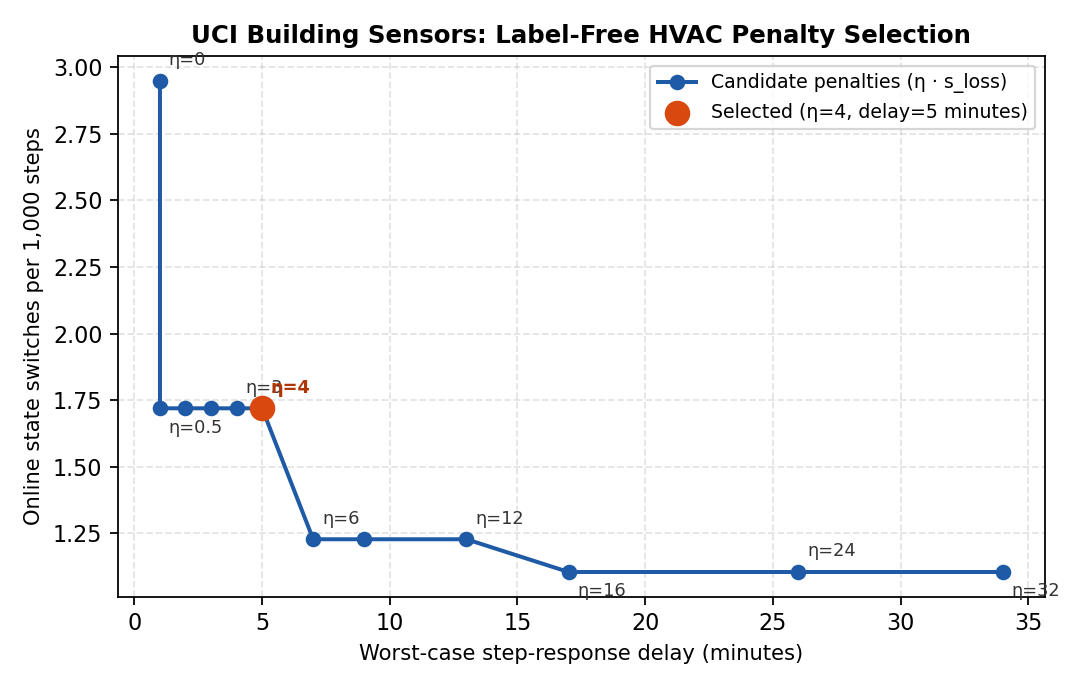
\includegraphics[width=0.49\textwidth]{../outputs/occupancy_pareto.png}\hfill
  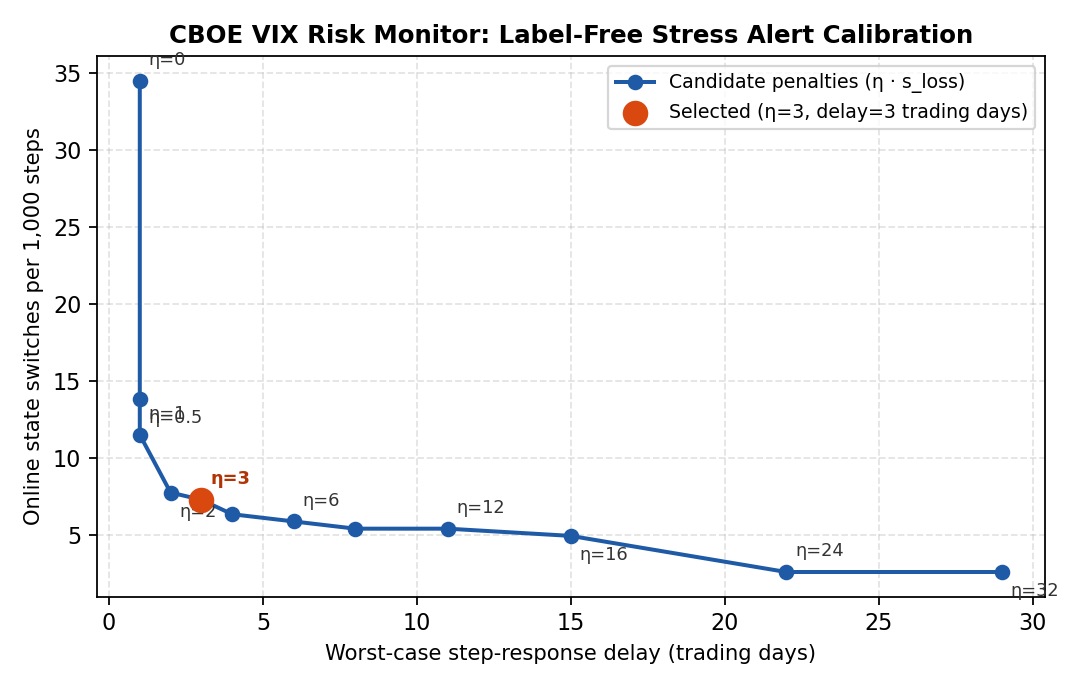
\includegraphics[width=0.49\textwidth]{../outputs/vix_pareto.png}
  \caption{Label-free Churn--Latency calibration curves on training streams for UCI Building Sensors (left, $B=5$ minutes) and CBOE VIX (right, $B=3$ trading days). Orange markers indicate the automatically selected penalty $\lambda = \eta s_{\mathrm{loss}}$.}
  \label{fig:pareto}
\end{figure}

\begin{figure}[t]
  \centering
  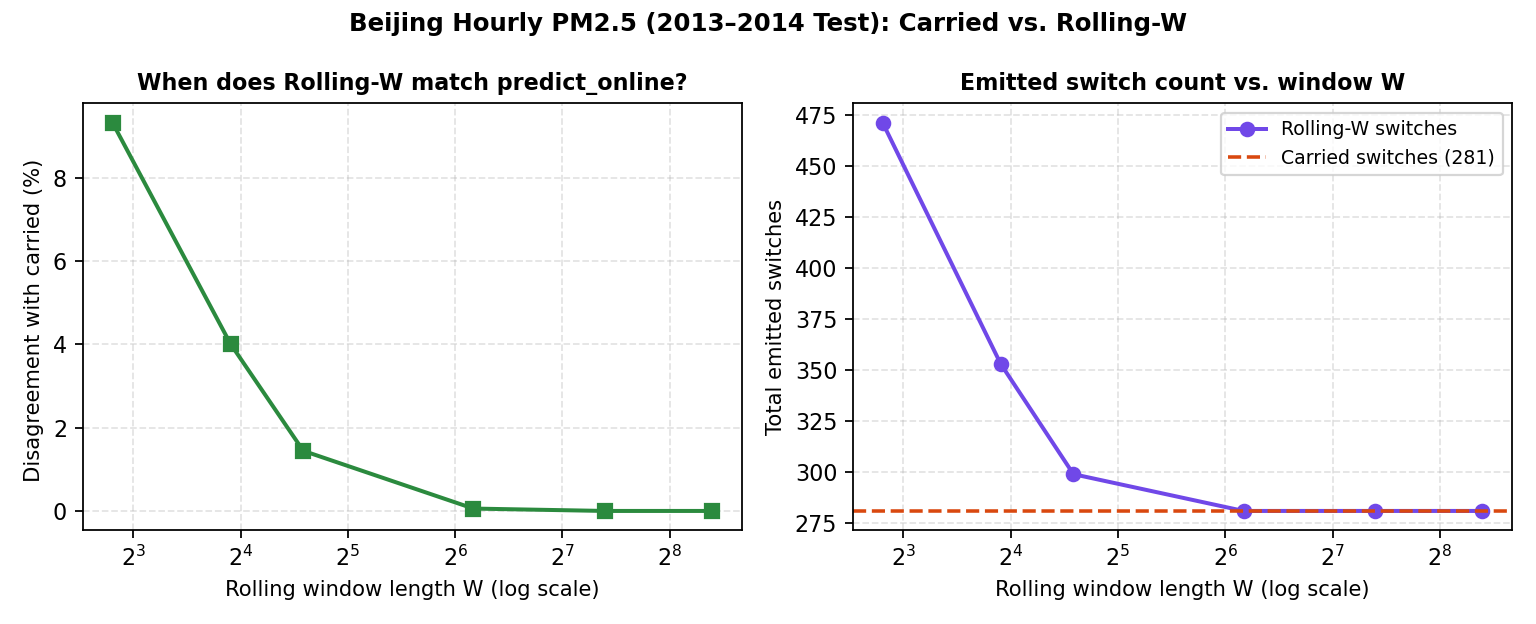
\includegraphics[width=0.92\textwidth]{../outputs/pm25_carried_vs_rolling.png}
  \caption{Empirical verification of Theorem~\ref{thm:coalescence} on $17,520$ out-of-sample hours of Beijing $\mathrm{PM}_{2.5}$ ($2013$--$2014$) at the selected penalty $\lambda = 11.14$. Short reset windows ($W=7$ hours) inflate alert switches from $281$ to $471$ ($+190$ spurious transitions), whereas windows $W \ge 168$ hours coalesce to $0.00\%$ disagreement with $O(1)$-memory carried-score decoding.}
  \label{fig:coalescence}
\end{figure}

Table~\ref{tab:summary} and Figures~\ref{fig:pareto}--\ref{fig:coalescence} summarize the empirical findings:
\begin{itemize}
  \item \textbf{Consistent $66\%$--$75\%$ churn reduction within delay budgets.} Across minute-level building sensors, hourly pollution telemetry, and daily market volatility, normalizing by $s_{\mathrm{loss}}$ selects $\eta \in \{3, 4\}$ purely from the delay ceiling $\lambda < B\Delta$, eliminating two-thirds to three-quarters of unpenalized switching noise out of sample.
  \item \textbf{Objective ground-truth validation on building sensors.} On the $12,417$ unseen UCI test minutes, unsupervised carried-score decoding cuts HVAC relay switches from $6.26$ to $1.62$ per day while retaining $83.92\%$ agreement with held-out camera occupancy labels and achieving a $1.0$-minute median empirical detection lag across sustained room-entry events (well within the $5$-minute worst-case budget).
  \item \textbf{Physical confirmation of short-window inflation and coalescence.} As predicted by Theorem~\ref{thm:coalescence}, resetting a short rolling window ($W = 7$) at the same $\lambda$ inflates out-of-sample transitions from $10$ to $24$ on UCI Test~2, from $281$ to $471$ ($+190$ extra switches) on Beijing $\mathrm{PM}_{2.5}$ (Figure~\ref{fig:coalescence}), and from $65$ to $111$ on VIX. Once $W$ exceeds the empirical barrier-hitting horizon ($W \ge 127$ min on Occupancy, $W \ge 168$ h on $\mathrm{PM}_{2.5}$, $W \ge 63$ d on VIX), disagreement between rolling-$W$ and carried-score decoding drops to \emph{identically $0.00\%$}.
\end{itemize}

\section{Conclusion and Limitations}

Separating real-time regime stabilization from financial return forecasting clarifies both the mathematics and practical engineering of Statistical Jump Models. For two-state models, causal dynamic programming is governed by a one-dimensional clipped accumulator whose barrier width $\lambda$ directly controls step-response latency via $\lambda < B\Delta$. Propagating this bounded score forward in $O(1)$ memory avoids the switching inflation of short reset windows while matching long rolling windows identically once saturation occurs.

Several limitations bound our conclusions. First, the closed-form delay expressions \eqref{eq:d01}--\eqref{eq:budget} measure deterministic step transitions between fitted prototypes $\mu_0$ and $\mu_1$; gradual drifts with $|g_t| < \Delta$ take proportionally longer to cross $\pm\lambda$. Second, while \texttt{jm-online} supports $K \ge 3$ states and continuous probability-simplex jump models numerically, exact scalar reduction applies specifically to $K = 2$. Extending analytical coalescence bounds to multi-state simplex decoders and streaming centroid adaptation under nonstationary drift are natural directions for follow-up work.

\paragraph{Acknowledgments and Reproducibility.}
The author thanks Professor Andrew Leahy and Knox College's Richter Memorial Fund for research guidance and support. All source code, unit tests, and benchmark reproduction scripts are available in the open-source \texttt{jm-online} repository. AI-assisted tools were used during software engineering, literature search, and manuscript editing; all mathematical proofs and empirical outputs were verified directly against executable tests and public datasets.

\begin{thebibliography}{99}

\bibitem{ag2009}
A.~E. Allahverdyan and A.~Galstyan.
\newblock On maximum a posteriori estimation of hidden {M}arkov processes.
\newblock In \emph{Proceedings of the Twenty-Fifth Conference on Uncertainty in Artificial Intelligence (UAI)}, pages 1--9, 2009.

\bibitem{behn1988}
U.~Behn and V.~A. Zagrebnov.
\newblock One-dimensional {M}arkovian-field {I}sing model: physical properties and characteristics of the discrete stochastic mapping.
\newblock \emph{Journal of Physics A: Mathematical and General}, 21(9):2151--2165, 1988.

\bibitem{bemporad2018}
A.~Bemporad, V.~Breschi, D.~Piga, and S.~P. Boyd.
\newblock Fitting jump models.
\newblock \emph{Automatica}, 96:11--21, 2018.

\bibitem{candanedo2016}
L.~M. Candanedo and V.~Feldheim.
\newblock Accurate occupancy detection of an office room from light, temperature, humidity and $\mathrm{CO}_2$ measurements using statistical learning models.
\newblock \emph{Energy and Buildings}, 112:28--39, 2016.

\bibitem{cortese2026}
F.~P. Cortese, P.~N. Kolm, and E.~Lindstr{\"o}m.
\newblock Generalized information criteria for high-dimensional sparse statistical jump models.
\newblock \emph{Statistical Methods \& Applications}, 2026.

\bibitem{cortese2024air}
F.~P. Cortese and A.~Pievatolo.
\newblock Statistical jump model for mixed-type data with missing data imputation.
\newblock \emph{arXiv preprint arXiv:2409.01208}, 2024.

\bibitem{liang2015}
X.~Liang, T.~Zou, B.~Guo, S.~Li, H.~Zhang, S.~Zhang, H.~Huang, and S.~X. Chen.
\newblock Assessing {B}eijing's $\mathrm{PM}_{2.5}$ pollution: severity, weather impact, {APEC} and winter heating.
\newblock \emph{Proceedings of the Royal Society A}, 471(2182):20150257, 2015.

\bibitem{nystrup2020}
P.~Nystrup, E.~Lindstr{\"o}m, and H.~Madsen.
\newblock Learning hidden {M}arkov models with persistent states by penalizing jumps.
\newblock \emph{Expert Systems with Applications}, 150:113307, 2020.

\bibitem{nystrup2021}
P.~Nystrup, P.~N. Kolm, and E.~Lindstr{\"o}m.
\newblock Feature selection in jump models.
\newblock \emph{Expert Systems with Applications}, 184:115558, 2021.

\bibitem{shu2024}
Y.~Shu, C.~Yu, and J.~M. Mulvey.
\newblock Downside risk reduction using regime-switching signals: A statistical jump model approach.
\newblock \emph{Journal of Asset Management}, 25:493--507, 2024.

\end{thebibliography}

\end{document}
